\chapter{ランダムウォークの固有値とエクスパンダーグラフ}
遷移確率行列$P \in [0,1]^{V \times V}$に従う$V$上の既約的かつ非周期的なランダムウォーク$(X_t)_{t\ge 0}$を考え,
その一意な定常分布を$\pi$とする.
\Cref{thm:random walk convergence}より収束性が保証されるが, その速さを遷移確率行列の固有値に基づいて評価するのが本チャプターの目標である.
この議論の土台となるのがランダムウォークの可逆性という概念である.
一般の遷移確率行列は対称とは限らないが, 可逆性を仮定することによって
遷移確率行列を対称行列として扱うことができ,
対称行列に対して展開される固有値分解などの理論を同じように
遷移確率行列に対しても適用することができる.
これに基づいて既約性, 非周期性, 可逆性を持つランダムウォークの混交時間の上界を与える.
また, エクスパンダーグラフの概念をそのグラフ上の単純ランダムウォークに基づいて定義し,
その組合せ論的な性質をいくつか紹介する.

\section{ランダムウォークの固有値と可逆性}
遷移確率行列$P \in [0,1]^{n \times n}$の固有値
\footnote{本講義では左固有値, すなわち$Px=\lambda x$を満たす$\lambda\in \Comp$を考える.}
$\lambda_1,\dots,\lambda_n$について考える.
全ての成分が$1$であるベクトル$\allone\in \Real^n$を考えると$P\allone = \allone$であるから
$P$は固有値$1$を持つことがわかる.
また, 以下の結果が知られている (Perron--Frobeniusの定理やGershgorinの定理から従う):
\begin{lemma}{遷移確率行列の固有値}{random walk eigenvalue}
    既約的かつ非周期的なランダムウォークの
    遷移確率行列$P\in [0,1]^{n\times n}$の固有値を$\lambda_1,\dots,\lambda_n$とすると,
    全ての$i\in\{1,\dots,n\}$に対して$\abs{\lambda_i} \le 1$を満たす.
    さらに,固有値$1$の多重度は$1$であり (つまり固有値$1$に対応する固有空間は$\{c\allone \colon c \in \Real\}$となる), 他の固有値は全て絶対値が真に$1$より小さい.
\end{lemma}
%

一方でこれまで見ていたグラフ上のランダムウォークは可逆性と呼ばれる嬉しい性質を持っており,
ある意味で対称行列のように扱うことができる.
\begin{definition}{可逆性}{reversible}
    遷移確率行列$P$を持つ$V$上のランダムウォークは,
    ある$V$上の分布$\pi \in [0,1]^V$が存在して
    \begin{align}
        \forall u,v\in V,\pi(u) P(u,v) = \pi(v) P(v,u) \label{eq:reversible}
    \end{align}
    を満たすとき\emph{可逆 (reversible)}であるという.
\end{definition}
\cref{eq:reversible}で表される条件を\emph{詳細釣り合い条件 (detailed balanced equation)}という.
分布$\pi\in [0,1]^V$を対角成分に並べた対角行列$\Pi\in[0,1]^{V\times V}$を用いると
$(\ref{eq:reversible}) \iff \Pi P = (\Pi P)^{\top}$
となる.

可逆性とは直感的に言うと, 逆再生しても同じ分布のランダムウォークになるという性質である.
ランダムウォーク$(X_t)_{t\ge 0}$であって初期頂点$X_0$が分布$\pi$に従って選ばれたものを考えよう.
適当な時刻$t=T$で打ち切って得られる頂点列$(X_0,\dots,X_T)$に対し, 順序を逆にした系列
$(X_T,\dots,X_0)$はランダムウォークから得られた系列と見做せるだろうか?
仮にこれがある遷移確率行列$P^*\in[0,1]^{V\times V}$に従うランダムウォークであったとしよう.
簡単のため$T=1$とする ($T\ge 2$に関しても同じ議論が適用できる).
初期頂点$X_0$の分布$\pi$が定常分布だとすると, $X_1$の分布も$\pi$である.
また, ランダムウォークの条件から$\Pr[X_1 = v \tand X_0=u] = \pi(u)P(u,v)$である.
従って条件付き確率の定義より
\begin{align}
    P^*(v,u) = \Pr[X_0 = u | X_1 = v] = \frac{\Pr[X_0 = u \tand X_1 = v]}{\Pr[X_1 = v]} = \frac{\pi(u)P(u,v)}{\pi(v)} \label{eq:reversal chain}
\end{align}
が得られる.
もし元のランダムウォークが可逆ならば, \cref{eq:reversible}から$P^*=P$を得る.
すなわち, ランダムウォークの可逆性とはそのランダムウォークが時間反転に関して対称性を持つことを意味する.
なお, \cref{eq:reversal chain}で得られる遷移確率行列に従って生成されるランダムウォークを\emph{時間反転ランダムウォーク (time-reversal random walk)}と呼ぶ.

\paragraph*{例1.単純ランダムウォーク}
連結グラフ$G=(V,E)$上の単純ランダムウォークを考えよう.
\cref{eq:SRW stationary distribution}で与えられる定常分布を$\pi$とすると
任意の二頂点$u,v\in V$に対して
\[
    \pi(u) P(u,v) = \frac{\deg(u)}{2|E|} \cdot \frac{\indicator{\{u,v\}\in E}}{\deg(u)}
    = \frac{\deg(v)}{2|E|} \cdot \frac{\indicator{\{u,v\}\in E}}{\deg(v)}
    = \pi(v) P(v,u)
\]
より, 単純ランダムウォークは可逆である (連結なので全ての頂点に対して$\deg(u)>0$である).
ここで, $\indicator{\dots}$は指示関数である.

\paragraph*{例2.重み付きランダムウォーク}
重みつきグラフ$G=(V,E,W)$上の重み付きランダムウォークを考えよう.
重み行列$W$の成分和を$S=\sum_{u,v\in V} W(u,v)$として
分布$\pi(u) = \frac{\deg_W(u)}{S}$を考えると,
\[
    \pi(u) P(u,v) = \frac{\deg_W(u)}{S} \cdot \frac{W(u,v)}{\deg_W(u)}
    = \frac{\deg_W(v)}{S} \cdot \frac{W(v,u)}{\deg_W(v)}
    = \pi(v) P(v,u)
\]
より, 可逆である.

\paragraph*{例3.有向グラフ上のランダムウォーク}
可逆で\emph{ない}例として次の遷移確率行列で与えられるランダムウォークを考えてみよう:
\begin{align*}
    P = \begin{pmatrix}
            0 & 1 & 0 \\
            0 & 0 & 1 \\
            1 & 0 & 0
        \end{pmatrix}.
\end{align*}
この例は遷移が決定的なのでランダムウォークとしては面白くないが,
次のようにして可逆でないことが確認できる:
頂点集合を$V=\{0,1,2\}$とし, $i\in V$に対して$(i+1)\bmod 3$を省略して$i+1 \in V$と書くと
\begin{align*}
    \pi(i) = \pi(i) P(i, i+1) = \pi(i+1)P(i+1,i) = 0
\end{align*}
より$\pi=0$となってしまい, 分布であることに矛盾.

\begin{exercise}{easy}{prob2}
    可逆なランダムウォークの遷移確率行列を$P$とする.
    \cref{eq:reversible}を満たす分布$\pi$は定常分布であることを示せ.
\end{exercise}

%


\section{定常分布から定まる内積とノルム}
可逆なランダムウォークは遷移確率行列の固有値を考える上で非常に扱いやすいランダムウォークのクラスとなっている.
ランダムウォークの分布は遷移確率$P$を右から掛けて得られるのに対し,
    固有値に基づく議論では左固有値を考えており,
この左右の差異に違和感を覚える読者もいるであろう.
実は可逆なランダムウォークでは遷移確率行列を対称行列のように扱うことができ,
ゆえに左右どちらから作用させようが本質的に同じとなる.
このことを説明するために, $\Real^V$に次の内積を導入する.
\begin{definition}{}{naiseki}
    有限集合$V$上の分布$\pi\in(0,1]^V$に対し,
    $\Real^V$に以下の内積$\piprod{\cdot,\cdot}$を定めた内積空間を$\pispace$で表す:
    \begin{align*}
        \piprod{f,g} \defeq \sum_{u \in V} \pi(u) f(u) g(u)
        = f^\top \Pi g.
    \end{align*}
    ここで$f,g$は列ベクトルとして扱い, $\Pi=\mathrm{diag}(\pi)$はベクトル$\pi$の成分を対角に並べた行列である.
    また, 内積$\piprod{\cdot,\cdot}$が誘導するノルムを$\pinorm{\cdot}$で表す.
    すなわち, $f\in\Real^V$に対して
    \[
        \pinorm{f} \defeq \sqrt{\piprod{f,f}}.
    \]
    %    二つのベクトル$f,g \in \Real^V$が$\piprod{f,g} = 0$であるとき, $f \piorth g$で表す.
\end{definition}
\cref{def:naiseki}で考える分布$\pi$は全ての成分が正であるため,
上記の内積$\piprod{\cdot,\cdot}$はちゃんと実ベクトル空間の内積の公理(対称双線形性, 非退化性, 半正定値性)を満たしており,
確かに$\pispace$は内積空間である.

$\Real^V$上の通常の内積$\abra{\cdot,\cdot}$を考えたとき, 任意の対称行列$M \in \Real^{V\times V}$とベクトル$f,g\in \Real^V$に対して $\abra{f,Ag} = \abra{Af,g}$
が成り立っていたが,
可逆なランダムウォークの遷移確率行列$P$は内積$\piprod{\cdot,\cdot}$に関して同様の性質を持つ.
\begin{lemma}{}{reversible adjoint}
    定常分布$\pi$をもつ可逆なランダムウォークの遷移確率行列$P$は,
    任意の$f,g\in\Real^V$に対して
    \[ \piprod{f,Pg} = \piprod{Pf,g} \]
    を満たす.
\end{lemma}
\begin{proof}
    定常分布$\pi$を対角成分に並べた対角行列$\Pi$を考えると
    \begin{align*}
        \piprod{f,Pg} & = f^\top \Pi P g                                              \\
                      & = f^\top (\Pi P)^\top g &  & \text{$\because$可逆性より$\Pi P$は対称} \\
                      & = (Pf)^\top \Pi g       &  & \text{$\because\Pi^\top = \Pi$}  \\
                      & = \piprod{Pf,g}.
    \end{align*}
\end{proof}
一般に$P$が可逆とは限らない場合,
\cref{eq:reversal chain}で与えられる時間反転ランダムウォークの遷移確率行列$P^*$に対し$\piprod{f,Pg} = \piprod{P^*f,g}$が成り立つ.
この意味で$P^*$は$P$の随伴とみなすことができる.


対称行列に対して展開される固有値分解などの理論は可逆なランダムウォークの遷移確率行列に対しても同様に展開できる.
例えば, 対称行列と同様に可逆なランダムウォークの遷移確率行列は実固有値をもつ.
\begin{lemma}{実固有値性}{reversible real eigenvalue}
    既約的かつ可逆なランダムウォークの遷移確率行列$P$と定常分布$\pi$に対し,
    行列
    \begin{align}
        A \defeq \sqrt{\Pi} P \sqrt{\Pi}^{-1} \label{eq: symmetrized P}
    \end{align}
    を考える.
    $P$と$A$は(多重度も含め)同じ固有値をもち, これらは全て実数である.
\end{lemma}
\begin{proof}
    行列$A$は対称である.
    実際,
    \begin{align*}
        A^\top & = \sqrt{\Pi}^{-1} P^{\top} \sqrt{\Pi}                            &  & \text{$\because$$\sqrt{\Pi},\sqrt{\Pi}^{-1}$は対称} \\
               & = \sqrt{\Pi} \cdot \Pi^{-1} P^{\top} \Pi \cdot \sqrt{\Pi}^{-1}                                                         \\
               & = \sqrt{\Pi} \cdot \Pi^{-1} (\Pi P)^{\top} \cdot \sqrt{\Pi}^{-1}                                                       \\
               & = \sqrt{\Pi} \cdot \Pi^{-1} \Pi P \cdot \sqrt{\Pi}^{-1}          &  & \text{$\because$可逆性より$\Pi P$は対称}                 \\
               & = A.
    \end{align*}
    $A$は対称なので全ての固有値は実数である.

    $A$の固有値$\lambda$に対する固有ベクトルを$x$とし, ベクトル$y\defeq \sqrt{\Pi}^{-1}x$を考える.
    固有ベクトルの式
    \begin{align*}
        A x = (\sqrt{\Pi} P \sqrt{\Pi}^{-1})x =  \lambda x
    \end{align*}
    の両辺に左から$\sqrt{\Pi}^{-1}$を掛けると
    \begin{align*}
        P y = \lambda y
    \end{align*}
    を得る.
    すなわち, $P$と$A$は同じ固有値を持つ.
    特に, $P$の固有値も全て実数である.
\end{proof}
\cref{lem:reversible real eigenvalue}において既約性の仮定は除去できる.
実際, $P$が定める状態遷移を表す有向グラフを強連結成分に分解し,
各成分ごとに\cref{lem:reversible real eigenvalue}を適用すればよい.

%
\begin{theorem}{固有分解}{eigendecomposition}
    既約的かつ可逆なランダムウォークの遷移確率行列を$P$とし, その定常分布を$\pi$とする.
    $|V|=n$とする.
    $P$の固有値を$1=\lambda_1\ge \dots \ge \lambda_n \ge -1$とする.
    空間$\pispace$の正規直交基底$x,\dots,x_n$が存在して任意の$t\ge 1$に対して
    \[ P^t\Pi^{-1} = \sum_{i=1}^n \lambda_i^t x_i x_i^{\top}  \]
    と表せ, さらに各$x_i$は$P$の固有値$\lambda_i$に対応する固有ベクトルとなる.
    
    特に$x_1 = \allone$であり,
    $J \in \Real^{V \times V}$を全成分が$1$の行列とすると
    \[ P^t \Pi^{-1} - J =  \sum_{i=2}^n \lambda_i^t x_i x_i^\top \]
    と表せる.
\end{theorem}
\begin{proof}
    \cref{eq: symmetrized P}で定義された行列$A$は対称なので,
    対称行列に対する固有分解の定理より,
    通常の内積$\abra{\cdot, \cdot}$の意味での$\Real^V$の正規直交基底$y_1,\dots,y_n$が存在して
    \[
        A = \sum_{i=1}^n \lambda_i y_i y_i^\top
    \]
    と表せ, さらに各$y_i$は$A$の固有値$\lambda_i$に対応する固有ベクトルとなる.
    一方で$A^t = \sqrt{\Pi} P^t \sqrt{\Pi}^{-1}$だから,
    \[
        \sqrt{\Pi} P^t \sqrt{\Pi}^{-1} = \sum_{i=1}^n \lambda_i^t y_i y_i^\top.
    \]
    両辺に左右から$\sqrt{\Pi}^{-1}$を一つずつ掛けて
    $x_i = \sqrt{\Pi}^{-1}y_i$とおくと
    \[
        P^t \Pi^{-1} = \sum_{i=1}^n \lambda_i^t x_i x_i^\top
    \]
    を得る.
    ここで
    \[
        \piprod{x_i,x_j} = \abra{\sqrt{\Pi}x_i,\sqrt{\Pi}x_j} = \abra{y_i,y_j} = \indicator{i=j}
    \]
    より, 確かに$(x_i)_{i=1,\dots,n}$は空間$\pispace$の正規直交基底である.
    さらに
    \[
        Px_i = P\sqrt{\Pi}^{-1}y_i = \sqrt{\Pi}^{-1}Ay_i = \lambda_i x_i
    \]
    より確かに$x_i$は$P$の固有値$\lambda_i$に対応する固有ベクトルである.

    特に, $\lambda_1=1$に対応する$A$の固有ベクトルは$y_1 = (\sqrt{\pi(u)})_{u \in V}$なので,
    対応する$P$の固有ベクトルは$x_1 = \allone$となる.
\end{proof}

空間$\pispace$上での期待値と分散を以下のように定義する:
\begin{definition}{期待値と分散}{expectation and variance}
    \cref{thm:eigendecomposition}と同じ仮定の下で,
    $f \in \pispace$の
    期待値と分散を
    \begin{align}
        &\Epi[f] \defeq \piprod{f,\allone} = \sum_{u\in V}\pi(u) f(u), \label{eq:mean}\\
        &\Varpi[f] \defeq \pinorm{f - \E_\pi[\allone]}^2 = \E_\pi [f^2] - (\E_\pi [f])^2 \label{eq:variance}
    \end{align}
    とする.
\end{definition}
すなわち, 関数$f\colon V \to \Real$を,
ランダムに選ばれた$u\sim \pi$に対して$f(u)$を出力する確率変数とみなして
その平均と分散をそれぞれ$\Epi[f],\Varpi[f]$とした.
以後, 特に混乱がない限り, $\Epi[f]$や$\Varpi[f]$は$\Epi f$や$\Varpi f$などとも表す.
同様に共分散$\mathrm{Cov}_\pi(f,g)$を$\piprod{f,g} - \Epi f \cdot \Epi g$で定義できるが,
この値は以下の性質を持つ.
\begin{lemma}{}{covariance}
    任意の$f,g\in \pispace$に対し,
    \[
        \abs*{\piprod{f,g} - \Epi f\cdot \Epi g} \le \sqrt{\Varpi f\cdot \Varpi g}.
    \]
\end{lemma}
\begin{proof}
    \cref{thm:eigendecomposition}で得られる$\pispace$の正規直交基底を$x_1,\dots,x_n$とし, 関数$f,g$をこれらの線形結合
    \begin{align*}
        f &= \Epi f \cdot \allone + \sum_{i=2}^n f_i x_i,\\
        g &= \Epi g \cdot \allone + \sum_{j=2}^n g_j x_j
    \end{align*}
    で表す.
    ここで$f_i = \piprod{f,x_i},g_j = \piprod{g,x_j}$であり,
    $x_1 = \allone$なので$f_1 = \Epi f,g_1 =  \Epi g$である.
    特に, 基底$(x_i)$の直交性より
    従って
    \begin{align*}
        \abs*{ \piprod{f,g} - \Epi f\cdot \Epi g} 
        &\le \sum_{i\ge 2} \abs{f_i}\abs{g_i} \\
        &\le \sqrt{\sum_{i\ge 2}f_i^2} \cdot \sqrt{\sum_{j\ge 2} g_j^2} & & \text{$\because$Cauchy--Schwarzの不等式}\\
        &= \sqrt{\Varpi f} \cdot \sqrt{\Varpi g}
    \end{align*}
    より主張を得る.
\end{proof}
%
\section{ランダムウォークのスペクトルと混交時間}
非自明な固有値が絶対値の意味で小さいときに混交時間が上から抑えられることを示す.
\begin{definition}{}{second eigenvalue}
    サイズ$n$の集合$V$上の可逆なランダムウォークを考え,
    その遷移確率行列$P$の固有値を$1=\lambda_1 \ge \dots \ge \lambda_n\ge -1$に対し,
    $\lambda(P) \defeq \max\cbra{\abs{\lambda_2},\abs{\lambda_n}}$とする.
    特に, $\gamma\defeq 1-\lambda(P)$を\emph{スペクトルギャップ (spectral gap)}と呼ぶ.
\end{definition}
先確率行列$P$を作用させると分散が減少する.
\begin{lemma}{}{variance}
    遷移確率行列$P$と関数$f \in \pispace$に対し
    \[
        (Pf)(u) \defeq \sum_{v\in V} P(u,v)f(v)
    \]
    とする. このとき,
    \begin{align*}
        &\Epi[Pf] = \Epi f, \\
        &\Varpi[Pf] \le \lambda(P)^2 \cdot \Varpi [f].        
    \end{align*}
\end{lemma}
証明は演習問題とする.
\begin{exercise}{}{Epi Pf = f}
    \cref{lem:variance}を証明せよ.
\end{exercise}
この補題の重要な系としてエクスパンダー混交補題と呼ばれる重要な結果を得る.
エクスパンダー混交補題については\cref{sec:expander pseudorandom}でより詳しく紹介する.
\begin{corollary}{可逆ランダムウォークに対するエクスパンダー混交補題}{general expander mixing lemma}
    可逆なランダムウォークの遷移確率行列$P$を考える.
    任意の関数$f,g\in\pispace$に対し,
    \[ \abs*{\piprod{f,Pg} - \Epi f \cdot \Epi g} \le \lambda(P)\cdot \sqrt{\Varpi f \cdot \Varpi g}.  \]
\end{corollary}
\begin{comment}
\begin{proof}
    \cref{thm:eigendecomposition}で得られる空間$\pispace$の正規直交基底$x_1,\dots,x_n$を考え,
    関数$f$をそれらの線形結合
    \[ f = \sum_{i=1}^n f_i x_i\]
    で表す (ここで$f_i = \piprod{f,x_i}$).
    %
    ここで, $x_1 = \allone$なので$f_1 = \E_\pi f$なので,
    両辺に左から$P$を掛けて移項すると
    \[
        Pf - \Epi[f] \allone  = \sum_{i=2}^n f_i P x_i = \sum_{i=2}^n \lambda_i f_i x_i
    \]
    を得る.
    両辺の$\pinorm{\cdot}$をとると, ピタゴラスの定理より
    \begin{align*}
        \pinorm{Pf - \Epi[f]\allone}^2 &= \sum_{i=2}^n f_i^2 \lambda_i^2 \\
        &\le \lambda(P)^2\cdot \sum_{i=2}^n f_i^2 \\
        &= \lambda(P)^2\cdot \pinorm{f - \Epi[f]\allone}^2 \\
        &= \lambda(P)^2\cdot \Varpi f
    \end{align*}
    を得る.
\end{proof}
\end{comment}
混交時間とスペクトルギャップの間には以下の関係が知られている:
\begin{lemma}{混交時間とスペクトルギャップ}{mixing time and spectral gap}
    集合$V$上の既約, 非周期的, 可逆なランダムウォークを考え,
    そのスペクトルギャップを$\gamma$とする.
    定常分布$\pi$に対し$\pimin = \min_{u\in V} \pi(u)$とすると,
    任意の初期分布に対して
    \[ \tmix(\varepsilon) \le\frac{\log\rbra*{\frac{1}{2\pimin\varepsilon}}}{\log(1/\lambda)}. \]
    特に, スペクトルギャップが$\gamma>0$のとき,
    $\tmix(\varepsilon) \le \frac{1}{\gamma}\log\rbra*{\frac{1}{2\pimin\varepsilon}}$.
\end{lemma}
%
\begin{proof}
    \cref{thm:eigendecomposition}の正規直交基底を$x_1,\dots,x_n$とする.
    ピタゴラスの定理より任意のベクトル$f \in \Real^V$は
    \[ \pinorm{f}^2 = \sum_{i=1}^n \piprod{f,x_i}^2 \]
    を満たす.
    特に, 頂点$u$を固定し$f$としてディラック測度$f=\delta_u$とすると
    \begin{align*}
        \pi(u) & = \pinorm{\delta_u}^2                                                           \\
               & = \sum_{i=1}^n \piprod{\delta_u,x_i}^2                                          \\
               & = \sum_{i=1}^n \pi(u)^2x_i(u)^2                                                 \\
               & = \pi(u)^2 + \pi(u)^2\sum_{i=2}^n x_i(u)^2 &  & \text{($\because x_1=\allone$)}
    \end{align*}
    を得る.
    特に, $\sum_{i=2}^n x_i(u)^2 = \frac{1}{\pi(u)} - 1 \le \frac{1}{\pi(u)}$である.

    ここで, \cref{thm:eigendecomposition}より, $P^t\Pi^{-1} - J$の第$(u,v)$成分に着目すると
    \begin{align*}
        \abs*{\frac{P^t(u,v)}{\pi(v)} - 1} & \le \sum_{i=2}^n \abs{\lambda_i}^t \abs{x_i(u)x_i(v)}                                                                           \\
                                           & \le \lambda^t \sum_{i=2}^n  \sqrt{\sum_{i=2}^n x_i(u)^2} \sqrt{\sum_{i=2}^n x_i(v)^2} &  & \text{$\because$Cauchy--Schwarzの不等式} \\
                                           & \le \frac{\lambda^t}{\sqrt{\pi(u)\pi(v)}}                                                                                       \\
                                           & \le \frac{\lambda^t}{\pimin}
    \end{align*}
    を得る.
    特に, 任意の頂点$u\in V$に対して
    \[
        \dtv\rbra*{P^t(u,\cdot),\pi} = \frac{1}{2}\sum_{v\in V} \abs*{P^t(u,v) - \pi(v)} \le \frac{\lambda^t}{2\pimin}
    \]
    なので, 任意の初期分布に対して混交時間は
    \[
        \tmix(\varepsilon) \le \inf\cbra*{t\ge 0\colon \frac{\lambda^t}{2\pimin} \le \varepsilon} \le \frac{\log\rbra*{\frac{1}{2\pimin\varepsilon}}}{\log(1/\lambda(P))} \le \frac{1}{\gamma}\log\rbra*{\frac{1}{2\pimin\varepsilon}}.
    \]
    最後の不等式では$\forall x\in \Real,x\le \e^{x-1}$を用いた.
\end{proof}

\section{エクスパンダーグラフ}
グラフ$G=(V,E)$は, 単純ランダムウォークの非自明な第二固有値$\lambda(P)$が小さいときにエクスパンダーであるという.
多くの文脈では通常, 正則グラフに対してのみエクスパンダー性が定義されるが
本講義では一般のグラフに対してエクスパンダー性を定義する.
\begin{definition}{エクスパンダー}{expander}
    グラフ $G=(V,E)$上の単純ランダムウォークの遷移確率行列$P$が$\lambda(P) \le \lambda$を満たすときグラフ$G$は\emph{$\lambda$-エクスパンダー ($\lambda$-expander)}という.
    また, $P$の第二固有値が$\lambda_2 \le \lambda$を満たすとき, グラフ$G$は\emph{片側$\lambda$-エクスパンダー (one-sided $\lambda$-expander)}という.
\end{definition}
本講義ではエクスパンダー性を持つ単体複体も取り扱うため,
エクスパンダー性を持つグラフのことを\emph{エクスパンダーグラフ}と呼んで区別する.

要するにグラフのエクスパンダー性とは単純ランダムウォークの混交時間が小さいという性質を意味する.
二部グラフは周期的であり特に最小固有値が$\lambda_{|V|}=-1$となるためこの意味ではエクスパンダーグラフになりえないが,
片側エクスパンダーであるならば
遅延単純ランダムウォークの混交時間は小さくなる.

ランダムウォークの混交時間が小さいとはランダムウォークが「すぐに混ざり合う」ことを意味する.
この「すぐに混ざり合う」性質から, ランダムウォーク$(X_t)_{t\ge 0}$が時刻$t$までに訪れた頂点の集合を$U_t = \cbra*{X_0,\dots,X_t}$とすると, $\abs{U_t}$はすぐに拡大(expand)していく.

\paragraph*{例1 完全グラフ.}
グラフ$\rbra*{V, \binom{V}{2}}$を\emph{完全グラフ (complete graph)}という.
$n$頂点完全グラフ上の単純ランダムウォークの遷移確率行列$P$は, 単位行列$I$と全成分が$1$の行列$J$を用いて
$P = \frac{1}{n-1}(J-I)$で表せる.
完全グラフは正則グラフなので定常分布$\pi$は$V$上の一様分布である.
第一固有値は$\allone$であり,
その他の固有ベクトル$x_i$($i\ge 2$)は全て$\allone$に直交し, 特に$Jx_i = 0$となる.
従って$P x_i = -\frac{1}{n-1}x_i$なので, $\lambda_1=1$, $\lambda_2=\dots=\lambda_n = -\frac{1}{n}$である.
よって, $n$頂点完全グラフは$(1/n)$-expanderであると同時に片側$(-1/n)$-エクスパンダーグラフである
($\lambda(P)$の定義では絶対値をつけているが片側エクスパンダー性の定義では絶対値をつけていないことに注意).
%
\paragraph*{例2 閉路グラフ.}
頂点数$n$の閉路グラフとは, 頂点集合$V=\cbra{v_1,\dots,v_n}$に対して
辺集合$E$が$E = \cbra{\cbra{v_1,v_2},\dots,\cbra{v_{n-1},v_n}, \cbra{v_n,v_1}}$で与えられるグラフ$(V,E)$である.
頂点数$n$が偶数のとき, 閉路グラフは二部グラフとなる.

ここでは$\omega = \exp\rbra*{\frac{2\pi \mathrm{i}}{n}}$を$1$の冪根とし,
頂点集合を$V=\cbra{\omega^i \colon i=0,\dots,n-1}$とし, 各辺を$\cbra{\omega^i,\omega^{i+1}}$で表す.
任意の関数$f\colon V\to \Real$に$P$を作用させると
\[ Pf(\omega^i) = \frac{f(\omega^{i-1}) + f(\omega^{i+1})}{2}\]
を得る.
関数$x_k\colon \omega^j \mapsto \omega^{kj}$を考えると,
$Px_k (\omega_j) = \frac{\omega^{k(j-1)} + \omega^{k(j+1)}}{2} = \frac{\omega^{-k}+\omega^{-k}}{2}\cdot x_k(\omega_j)$を得る.
従って各$k=0,\dots,n-1$に対し$x_k$はそれぞれ固有値$\frac{\omega^k + \omega^{-k}}{2} = \cos\frac{2\pi k}{n}$に対応する固有ベクトルである.

これらの固有値を降順に並べて$1=\lambda_1\ge \dots\ge \lambda_n\ge-1$とすると,
$\lambda_2 = \cos\frac{2\pi}{n} = 1-\frac{4\pi^2}{2n^2} + O(n^{-4})$である.
頂点数$n$が偶数のときは$\lambda_n = -1$,
頂点数$n$が奇数のときは$\lambda_n = \cos\pi\rbra*{1 - \frac{1}{n}} = -\cos\frac{\pi}{n} = -1 + \frac{\pi^2}{2n^2} - O(n^{-4})$である.
従って頂点数$n$が奇数のときの閉路グラフは$\cos\frac{\pi}{n}$-エクスパンダーであり,
$n\to\infty$の漸近を考えると$n$のスペクトルギャップは$\Theta(1/n^2)$となる.

\subsection{エクスパンダー性の限界とラマヌジャングラフ(*)}
ランダムウォークがすぐに混ざり合うということはそのグラフは多くの辺を持つべきである.
例えば完全グラフは非常に強いエクスパンダー性を持つ一方で閉路グラフのエクスパンダー性は乏しい.
では, グラフの辺数を固定したとき, エクスパンダー性のパラメータ$\lambda$はどこまで小さくできるだろうか?
ここでは厳密な証明は与えずに直感的な議論によって正則グラフに絞ってエクスパンダー性の限界を説明する.

あとの節(\cref{sec:expander graph application})で詳しく述べるが,
応用上は正則なエクスパンダーグラフが重要である.
正則グラフ上のランダムウォークの遷移確率行列は単に隣接固有値を次数で割ったものであり定常分布も一様分布なので
単に隣接行列の固有値を考えれば良いことがわかる.\footnote{この理由からエクスパンダーグラフの理論は多くの教科書では正則グラフ上でのみ展開されるが, 本講義では一般のグラフ, ひいては一般のランダムウォークに対して展開している.}

固定した自然数$d\ge 3$に対して最もエクスパンダー性の強い(つまり$\lambda$が最小となる)$d$-正則グラフはどのようなグラフだろうか?
問題を言い換えればランダムウォークがより多くの頂点を訪れやすくするにはグラフをどのように構成すれば良いだろうか?

\paragraph*{理想的なグラフ: $d$-正則無限木.}
直感的な議論だが, 短い閉路があるとそれに沿って同じ頂点を訪れてしまうので, そのような閉路はない方が良いと思われる.
従ってそのグラフを虫眼鏡でズームすると局所的には木構造になっているべきであろう.
そこで「理想的な」グラフとして$d$-正則で頂点数が無限の木$T$を考える.
頂点集合$V$は加算無限であるため, 有限グラフに対する隣接行列や固有値の概念を無限グラフに拡張したものが必要である.
集合$\ell^2(V) \subseteq \Real^V$を
$\ell^2(V) = \cbra*{ f \colon V \to \Real\colon \sum_{u\in V}f(u)^2 < \infty }$とする.
隣接作用素$A\colon \ell^2(V) \to \ell^2(V)$を
\[
    A f(u) = \sum_{v \in N_T(u)} f(v)
\]
で定める. ここで$N_T(u)\subseteq V$は$T$において$u$と隣接している頂点の集合であり, $T$の$d$-正則性から
有限集合である.
作用素$A$のスペクトルを
\[
    \mathrm{spec}(A) = \cbra*{ \lambda \in \Real \colon A - \lambda I\text{ は可逆でない}}
\]
とする.
\begin{theorem}{}{infinite d-regular tree spectral}
    $d$-正則無限木$T$の隣接作用素$A$のスペクトルは以下を満たす:
        \[ \mathrm{spec}(A) \subseteq [-2\sqrt{d-1}, 2\sqrt{d-1}].\]
\end{theorem}
従って, 理想的なグラフを考えるとその隣接行列の非自明な固有値はその絶対値が高々$2\sqrt{d-1}$である
(第一固有ベクトル$\allone$に対応する関数は$\ell^2(V)$に属さない).
よって任意の$d$-正則グラフは$\lambda(P)\ge \frac{2\sqrt{d-1}}{d}$を満たすであろうことが予想される.

\paragraph*{Alon-Boppanaの定理.}
定数次数の正則グラフの直径は$\Omega(\log n)$を満たす.
\begin{lemma}{}{regular graph diameter}
    $d\ge 3$のとき,
    $n$頂点$d$-正則連結グラフ$G=(V,E)$の直径は$\diam(G) \ge \log_{d-1}\frac{(d-2)(n-1)}{d}$を満たす.
\end{lemma}
\begin{proof}
    頂点$u\in V$を固定すると, $u$から$\ell$本以下の辺を辿って辿り着ける頂点は高々
    \[ 1 + d + d(d-1) + \dots + d(d-1)^{\ell-1} \le 1 + d(d-1)^{\ell-1}\sum_{i=0}^{\ell-1}\rbra*{\frac{1}{d-1}}^i \le 1+\frac{d(d-1)^\ell}{d-2}  \]
    この値が$n$より真に大きいとき, $u$から$\ell$本以下の辺を辿って辿り着けない頂点が存在し, これは$\diam(G) \ge \ell$を意味する.
これを解くと$\ell > \log_{d-1}\frac{(d-2)(n-1)}{d}$を得る.
\end{proof}

\begin{theorem}{Alon--Boppanaの定理}{Alon Boppana}
    ある定数$c>0$が存在し, 任意の$n$頂点$d$正則グラフ$G$上の単純ランダムウォークの遷移確率行列$P$の第二固有値$\lambda_2$は
    \[ \lambda_2 \ge \frac{2\sqrt{d-1}}{d}\rbra*{ 1 - \frac{c}{\diam(G)^2}} \]
    を満たす.
\end{theorem}
特に, \cref{lem:regular graph diameter}より, 次数$d\ge 3$を固定して頂点数$n\to\infty$の漸近において$\ell = \Omega(\log n)$であるため, $\lambda_2 \ge \frac{2\sqrt{d-1}}{d} (1 - O(1/\log^2 n))$を満たす.
この結果は次数$d$を固定したときの正則グラフのエクスパンダー性のパラメータの限界を表している.

ここでは少し弱い下界として
\begin{align}
    \lambda_2 \ge \frac{2\sqrt{d-1}}{d}\rbra*{1 - O\rbra*{\frac{\log \diam(G)}{\diam(G)}}} \label{eq:weak alon boppana bound}
\end{align}
を証明する. この下界でも$\lambda_2 \ge \frac{2\sqrt{d-1}}{d}(1-o(1))$を示すには十分である.
\begin{proof}[\textbf{\cref{eq:weak alon boppana bound}の証明.}]
    遷移確率行列を$P$とし, 隣接行列を$A$とする.
    二頂点$u,v$を$uv$間の最短路が$\diam(G)$に等しくなるように固定し
    関数$f \colon V \to \Real$を$f = \delta_s - \delta_t$とすると, 任意の$k\ge 1$に対して
    \begin{align*}
        \lambda(P^{2k}) &= \lambda(P^k)^2 \\
        &\ge \frac{\Varpi[P^{k}f]}{\Varpi[f]} & & \text{$\because$\cref{lem:variance}}\\
        &= \frac{\pinorm{P^{k}f}^2}{\pinorm{f}^2} & & \text{$\because \Epi f=\Epi[P^{k}f] =0$} \\
        &= \frac{\piprod{f,P^{2k} f}}{\pinorm{f}^2} & & \text{$\because$\cref{lem:reversible adjoint}}\\
        &= \frac{P^{2k}(u,u) + P^{2k}(v,v) - 2P^{2k}(u,v)}{2} \\
        &= \frac{A^{2k}(u,u) + A^{2k}(v,v) - 2A^{2k}(u,v)}{2d^{2k}}. & & \text{$\because P=\frac{1}{d}A$}
    \end{align*}
    \cref{lem:adjacency walk count}より, $k=\floor*{\frac{\diam(G)-1}{2}}$とすると, $u,v$の選び方より$A^{2k}(u,v)=0$である.
    \cref{lem:adjacency walk count}より, $A^{2k}(u,u)$は頂点$u$を含む長さ$2k$の閉路の個数に等しい.

    \begin{lemma}{正則グラフの閉路数の下界}{closed walk regular graph}
        $d\ge 3$に対し, $T$を$d$-正則無限木とし, 頂点を一つ固定する.
        この頂点を含む長さ$2k$の閉路の個数を$t_{2k}$とすると
        \[ t_{2k} = d(d-1)^{k-1}\cdot \frac{1}{k+1}\binom{2k}{k} \]
        である.
        さらに,
        任意の$d$-正則グラフ$G=(V,E)$の任意の頂点$u$に対し, $u$を含む長さ$2k$の閉路の個数は少なくとも$t_{2k}$である.
    \end{lemma}

    まずは\cref{lem:closed walk regular graph}を認めて\cref{thm:Alon Boppana}の証明を完成させる (\cref{lem:closed walk regular graph}は後で証明する).
    二項係数$\binom{2k}{k}$はStirlingの近似により$\binom{2k}{k} \ge \frac{4^k}{\sqrt{\pi k}}\rbra*{1-\frac{1}{8k}}$を満たすことが示せる.
    従って, \cref{lem:closed walk regular graph}より,
    \begin{align*}
        \lambda(P)^{2k} &\ge d^{-2k} t_{2k} \\
        &\ge d^{-2k}\cdot (d-1)^k \cdot \frac{2^{2k}}{(k+1)\sqrt{\pi k}}\rbra*{1-\frac{1}{8k}}.
    \end{align*}
    特に, ある定数$c>0$が存在して
    \begin{align*}
        \lambda(P) &\ge \frac{2\sqrt{d-1}}{d} \cdot k^{-c/k} \\
        & \ge \frac{2\sqrt{d-1}}{d}\cdot \rbra*{1-O\rbra*{\frac{\log k}{k}}}.
    \end{align*}
    最後の不等号は$k^{-k}=\e^{-\frac{\log k}{k}} = 1-O\rbra*{\frac{\log k}{k}}$を用いた.
    $k=\floor*{\frac{\diam(G)-1}{2}}$を代入すれば\cref{eq:weak alon boppana bound}を得る.
\end{proof}
最後に\cref{lem:closed walk regular graph}を証明する.
\begin{proof}[\textbf{\cref{lem:closed walk regular graph}の証明.}]
    $d$-正則無限木$T$の特別な頂点$v_0$を一つ固定し, (グラフ理論においてスタンダードな)幾つかの用語を定義する.
    固定した特別な頂点$v_0$を\emph{根 (root)}と呼び,
    $T$の頂点$v$に対し, $\dist(v_0,v)$を\emph{深さ (depth)}と呼び$\mathrm{depth}(v)$で表す (特に$\mathrm{depth}(v_0)=0$である).
    頂点$v$に$T$上で隣接している$d$個の頂点からなる集合を$N_T(v)$と表す ($N_T(v)$に$v$は含めない).
    これらの隣接頂点のうち, 深さが$\mathrm{depth}(v)-1$となるただ一つの頂点を$v$の\emph{親 (parent)}と呼び,
    残りの深さ$\mathrm{depth}(v)+1$の頂点を$v$の\emph{子 (child)}と呼ぶ.

    \begin{figure}
        \begin{center}
        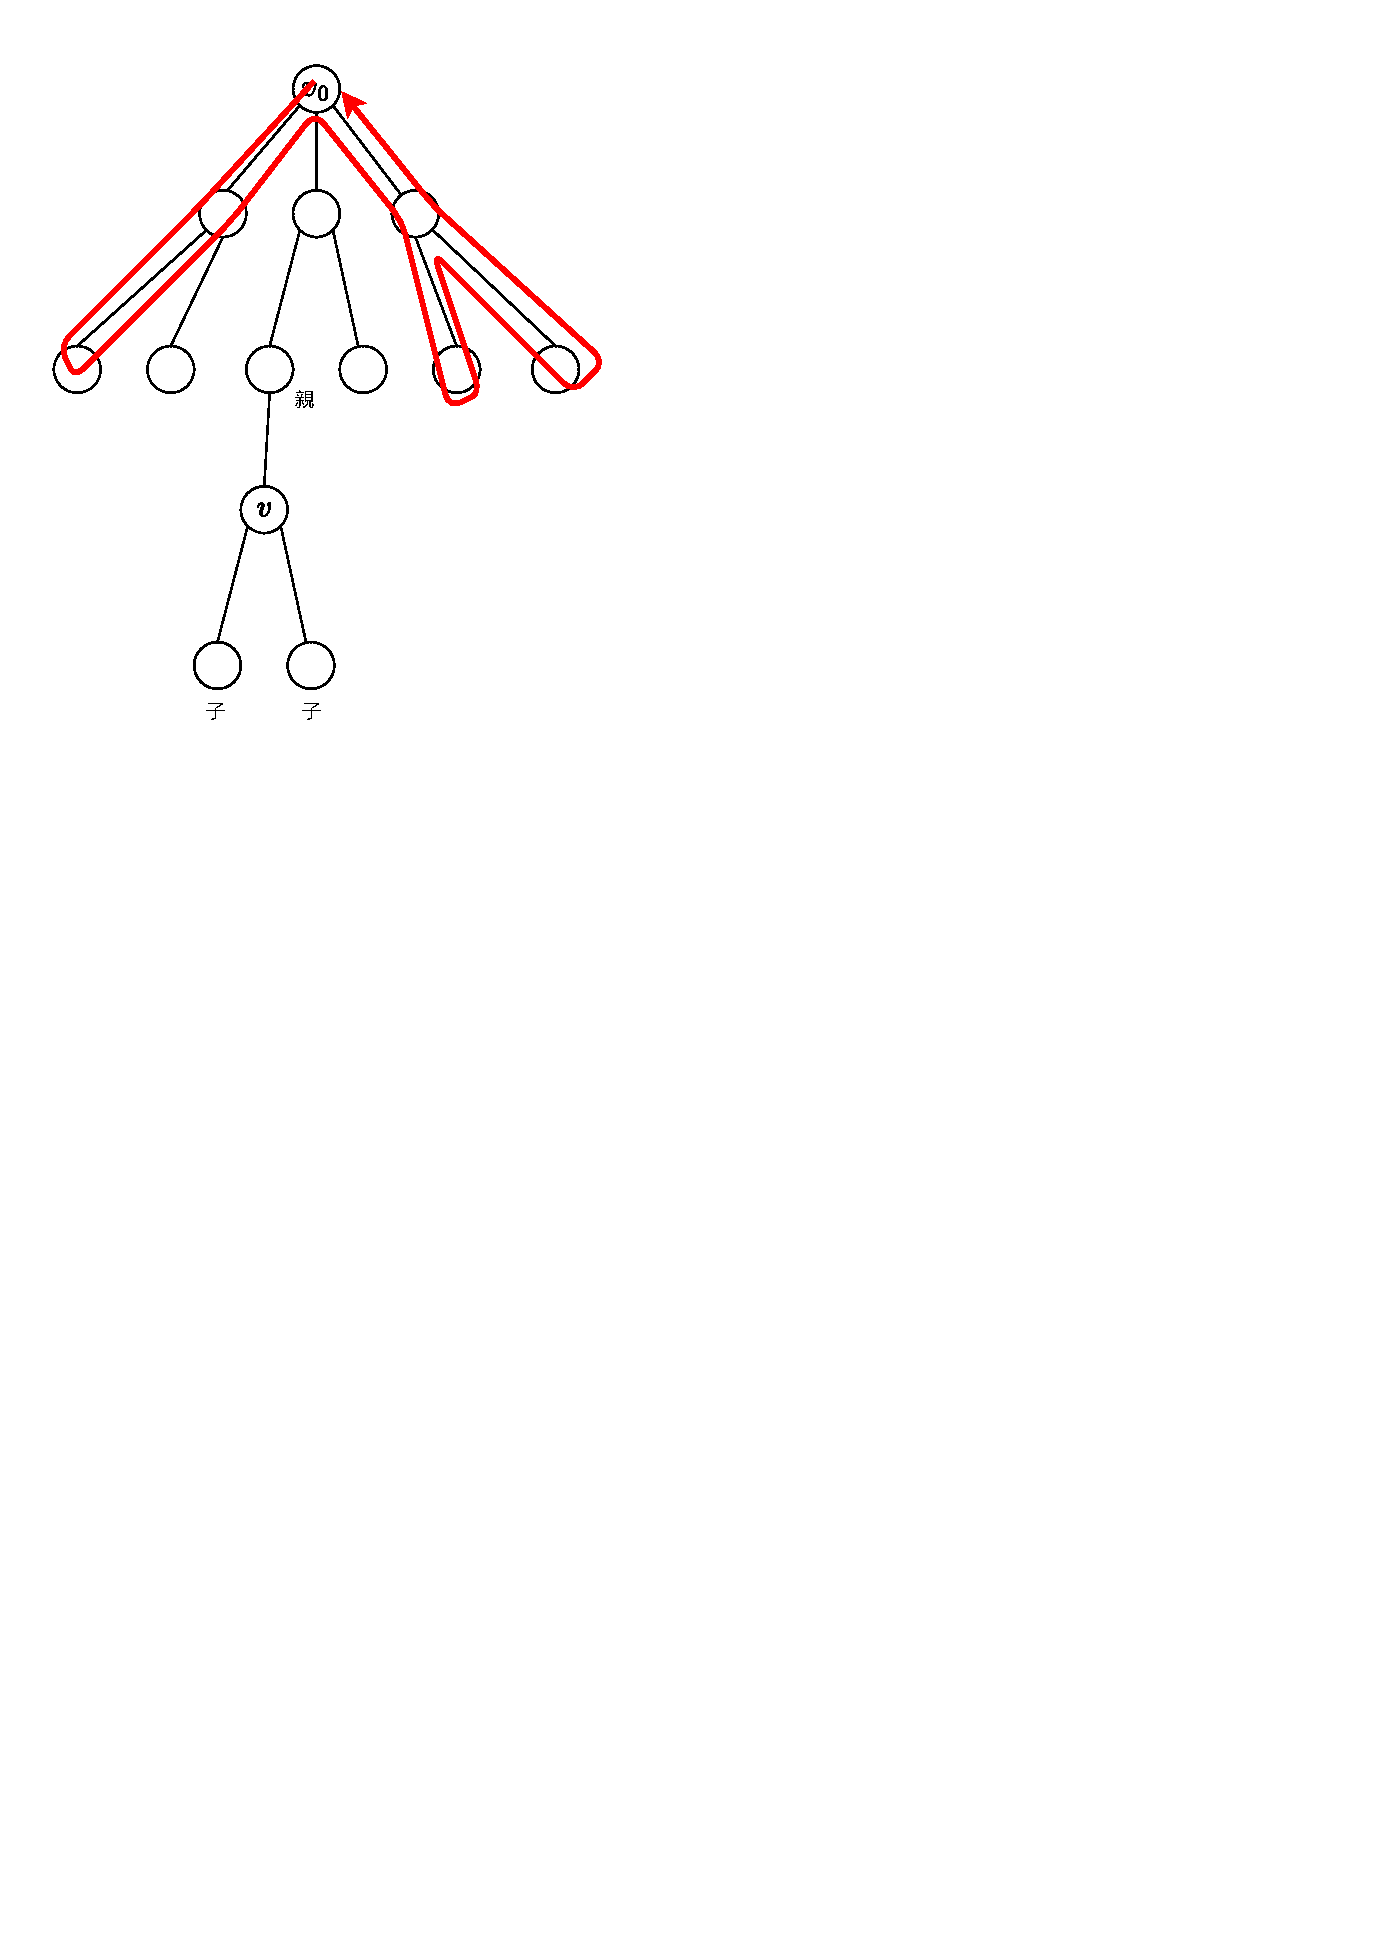
\includegraphics[width=8cm]{images/tree.pdf}
        \caption{$3$正則木$T$上の長さ$10$の閉路. 親から子への遷移と子から親への遷移を$5$回ずつ行う.}
        \end{center}
    \end{figure}
    
    木$T$において根を始点とする長さ$2k$の閉路$(v_0,\dots,v_{2k})$を考える (ここで$v_0=v_{2k}$).
    各$i$に対して$d_i = \mathrm{depth}(v_i)$とし, 列$(d_0,\dots,d_{2k})$を考える.
    まず$d_0=0$であり, その後は$d_{i+1} \in \cbra{d_i \pm 1}$であり, 常に非負性を保ちながら最後に$d_{2k}=0$となる.
    このような列$(d_0,\dots,d_{2k})$の総数はカタラン数と等しく, $\frac{1}{k+1}\binom{2k}{k}$に等しい.
    特に, 各$d_i - d_{i-1}$の符号を見ると$d_0 = d_{2k} = 0$より正と負がそれぞれ$k$個ずつ含まれている.

    次に, 各$(d_1,\dots,d_{2k})$に対して深さの履歴がこれと等しくなるような閉路の個数を考える.
    まず, $i=1$において, 頂点$v_0$からは子に遷移するため$v_1$の取り方は$d$通りある.
    各$i\ge 2$において, $d_i=d_{i-1}+1$ (すなわち$v_i$が$v_{i-1}$の子である)とき, $v_i$の選び方は$d-1$通りある.
    一方で親に遷移する場合はその遷移先は一意である.
    子への遷移はちょうど$k$回発生するため, 深さの履歴が与えられた$(d_1,\dots,d_{2k})$に等しくなるような閉路の個数は$d(d-1)^{k-1}$に等しい.
    従って$t_{2k} = \frac{1}{k+1}\binom{2k}{k} \cdot d(d-1)^{k-1}$を得る.

    後半の主張を証明する.
    $d$-正則グラフ$G$の頂点$u_0$を一つ固定する.
    木$T$の頂点集合を$U$, グラフ$G$の頂点集合を$V$とし,
    $N_T$の定義と同様にグラフ$G$の頂点$v \in V$に対しその$d$個の隣接頂点の集合を$N_G(v)$で表す.
    $G$から$T$への準同型写像$\phi \colon U \to V$を以下のように構成する\footnote{グラフ$G=(V,E)$から$H=(W,F)$への\emph{準同型写像 (homomorphism)}とは, 写像$\phi\colon V\to W$であって$\{u,v\}\in E\Rightarrow \{\phi(u),\phi(v)\}\in F$を満たすものである. ここでは自然に無限グラフに対してこの概念を拡張している.}:
        深さに関して帰納的に定義する.
        \begin{itemize}
        \item まず, $\phi(v_0) = u_0$とする.
        根$v_0$の子$N_T(v_0)$から$N_G(u_0)$への全単射$\phi_0$を任意に一つ選び,
        $\phi\colon N_T(v_0) \ni v' \mapsto \phi_1(v') \in N_T(u_0)$
        によって$N_T(v_0)$における$\phi$を定義する.
        \item $T$における深さ$\ell$以下の全ての頂点に対し$\phi(v)$が定義されているとする. 深さ$\ell$の各頂点$v$に対し, その親を$p$, 子を$c_1,\dots,c_{d-1}$とする. $v$とその親$p$に対しては$u\defeq \phi(v)$, $u_p\defeq \phi(p)\in U$が定義されている. このとき, 全単射$\psi\colon N_T(v)\setminus \{p\} \to N_G(u)\setminus\{u_p\}$を任意に一つ固定し, 各$\phi(c_j)$を$\psi(c_j)\in V$とする.
        \end{itemize}
    このようにして定義された写像$\phi\colon U \to V$は確かに準同型である.
    従って$T$の閉路$(v_0,\dots,v_{2k})$に対して$(\phi(v_0),\dots,\phi(v_{2k}))$は$G$の閉路になっている.
    さらに, $(\phi(v_0),\dots,\phi(v_{2k}))$の形になっている$G$の閉路が与えられたとき, $v_0$は一意に定まり, 以降の$v_i$は$\phi$の帰納的な定義で用いた全単射の逆写像を用いて順番に復元することができるため, $(v_0,\dots,v_{2k}) \mapsto (\phi(v_0),\dots,\phi(v_{2k}))$は単射である.
        従ってグラフ$G$に含まれるある頂点を始点とした長さ$2k$の閉路の個数は少なくとも$t_{2k}$である.
\end{proof}


\paragraph*{ラマヌジャングラフ.}
漸近的に\cref{thm:Alon Boppana}を達成するグラフを\emph{ラマヌジャングラフ (Ramanujan graph)}という.
\begin{definition}{ラマヌジャングラフ}{Ramanujan graph}
    $d$-正則グラフ$G=(V,E)$は, その単純ランダムウォークの遷移確率行列$P$の第二固有値$\lambda_2$が$\lambda_2 \le 2\sqrt{d-1}$を満たすとき, \emph{ラマヌジャングラフ (Ramanujan graph)}という.
\end{definition}

\cref{thm:Alon Boppana}を達成するグラフ列, すなわち,
次数$d$を固定したときに頂点数が増大していくグラフ列$(G_n)_{n\in\Nat}$であって各$G_n$が$d$-正則ラマヌジャングラフとなるものは存在
するだろうか?
この漸近的に最適な正則エクスパンダーグラフの構成は\citet{LPS88}によって初めてその構成が与えられた.
彼らは$d-1$が$4$で割った余りが$1$となる素数であるときに$d$-正則ラマヌジャングラフの列を構成した.
なお, 「ラマヌジャングラフ」という名称は\cite{LPS88}の証明がラマヌジャン予想と呼ばれる予想に依拠しているからである
(「予想」と書いたが当時は既に解決している).
%また, \cite{LPS88}とは独立同時期に\citet{Mar88}もラマヌジャングラフの族を構成しているようである
%    (元論文はロシア語で書かれており, 英語に翻訳されたものもあるようなのだが見つけることはできなかった).

\paragraph*{ランダム正則グラフ.}
\citet{LPS88}やその後続研究によりラマヌジャングラフ列については様々な構成方法が知られている.
では, そもそもラマヌジャングラフは何個あるのだろうか?
$n$頂点$d$-正則グラフ全体の集合を$\calG_{n,d}$とし,
    $\calG_{n,d}$から一様ランダムに選ばれたグラフ$G\sim\calG_{n,d}$を考える
    ($nd$は常に偶数とする).
この確率変数をランダム正則グラフという.
ランダム正則グラフは「ほぼ」ラマヌジャングラフであることが知られている
    \cite{Friedman_random_regular}.
\begin{theorem}{Friedmanの定理}{random regular graph Ramanujan}
    任意の$d\ge 3$と任意の$\varepsilon > 0$に対し,
    \[ \lim_{n\to\infty}\Pr\sbra*{\lambda(P) \ge \frac{2\sqrt{d-1}}{d} + \varepsilon} = 0. \]
\end{theorem}
すなわち, ほとんど全ての定数次数正則グラフはラマヌジャングラフと同等のスペクトルを持つ.

\subsection{エクスパンダーの擬似ランダム性(*)} \label{sec:expander pseudorandom}
この節は高次元エクスパンダーの本筋から少し外れるが,
エクスパンダーグラフの重要であることの理由の一つとしてその擬似ランダム性について概説する.

加法的組合せ論や計算量理論では\emph{擬似ランダム性 (pseudorandomness)}と呼ばれる概念が非常に重要な役割を果たしている.
\begin{definition}{分布の擬似ランダム性}{pseudorandomness}
    有限集合$\Omega$上のある分布$\mu$と関数族$\mathcal{F}=\{f\colon \Omega \to \binset\}$を考える.
    分布$\mu$は,
    任意の$f\in \mathcal{F}$に対して
    \[ \abs*{\E_{x\sim \mu} [f(x)] - \E_{y\sim U_{\Omega}}[f(y)]} \le \varepsilon\]
    を満たすとき, \emph{$\mathcal{F}$に対して$\varepsilon$-擬似ランダムである}という (ここで, $y\sim U_\Omega$とは$\Omega$上一様ランダムに$y$が選ばれたことを意味する).
\end{definition}
直感的には, 分布が擬似ランダムであるとは, その分布が任意の$f\in \mathcal{F}$を使っても一様分布と\emph{識別できない (indistinguishable)}ことを意味する.
例えば全変動距離に関する\cref{prop:dtv}では, $\mathcal{F}$を$V$上の二値関数全体 (すなわち任意の$V$の部分集合)の族としたときの識別不可能性のパラメータ$\varepsilon$が全変動距離で与えられることを意味する.
すなわち$\mu$は常に$\dtv(\mu,U_{\Omega}))$-擬似ランダムである.
関数クラス$\mathcal{F}$をより制限したときにパラメータ$\varepsilon$がどこまで小さくなるかに興味がある.

組合せ論では$\mathcal{F}$としてある特殊な関数クラスを仮定することによって\emph{組合せ論的擬似ランダム性}を定義する.
例えばグラフ理論や加法的組合せ論のコーナーストーンの一つと呼ばれるSzemerédiの正則化補題と呼ばれる結果は, 非常に大雑把に言えば
任意の密なグラフが定数個の擬似ランダムな二部グラフと疎な部分に分解できることを主張する定理である.
組合せ論的擬似ランダムネスの概念は特に加法的組合せ論において非常な協力な道具となっており,
Green--Taoの定理の証明においても重要な役割を果たしている
(驚くべきことに, 識別不可能性の枠組みでGreen--Taoの定理の証明を理解してそれを学習理論におけるブースティングの証明に応用するという研究もなされている!).

計算量理論では$\mathcal{F}$を「効率的なアルゴリズムの全体」や「素子数の少ない論理回路の全体」とすることで\emph{計算量的擬似ランダム性}を定義できる.
任意の効率的なアルゴリズムに対して一様ランダムな文字列と識別できないということは, その分布に従って生成されたメッセージを盗み見てもそこから得られる情報が何もない (ランダムな文字列を見てるのと同じ) であることから, 計算量的擬似ランダム性は暗号の計算量的安全性の定義の根幹をなすことがわかる.

エクスパンダーグラフの組合せ論的擬似ランダム性を説明する.
正則$\lambda$-エクスパンダー$G=(V,E)$を考える.
集合$\Omega=V\times V$上の分布$\mu = \mu_G$として
一様ランダムな辺$\{u,v\}\in E$を選び, $(u,v)$もしくは$(v,u)$どちらかを等確率で選んだ時の頂点対の分布とする.
すなわち,
\begin{align}
    \Pr_{(u,v)\sim \mu}\sbra*{ (u,v) = (s,t)} = \frac{\indicator{\{s,t\}\in E}}{2\abs{E}} = \frac{\indicator{\{s,t\}\in E}}{nd} \label{eq:expander mu}
\end{align}
とする.
関数族$\mathcal{F}$を
\begin{align}
    \mathcal{F} = \cbra*{ f_{S,T} \colon (s,t) \mapsto \indicator{s\in S,t\in T} \colon S,T\subseteq V}  \label{eq:expander F}
\end{align}
で定める.
%
\begin{lemma}{エクスパンダー混交補題}{expander mixing lemma}
    グラフ$G$が$n$頂点$d$-正則$\lambda$-エクスパンダーであるとき, \cref{eq:expander mu}で定義された分布$\mu$は\cref{eq:expander F}で定義された関数族$\mathcal{F}$に関して$\varepsilon$-擬似ランダムである.
    すなわち, 任意の頂点部分集合$S,T\subseteq V$に対して,
    $e(S,T) = \sum_{s\in S,t\in T} \indicator{\{s,t\} \in E}$を$S,T$間の辺の本数($S\cap T$内の辺は2回数える)とすると,
    \[
        \abs*{e(S,T) - \frac{d}{n}|S||T|} \le d\lambda\sqrt{|S||T|\rbra*{1-\frac{|S|}{n}}\rbra*{1-\frac{|T|}{n}}}.
    \]
\end{lemma}
%
グラフ$G$の隣接行列$A$を考えるとイメージしやすい.
この行列は全部で$nd$個の$1$を持っているため, 全成分の中で$1$の密度は$\frac{d}{n}$である.
ここで, 部分集合$S,T\subseteq V$に対して$A$の$S\times T$で定まる部分行列$A_{S,T}$を考える.
この行列に含まれる$1$の個数($e(S,T)$に等しい)は, $\frac{d}{n}\cdot |S||T|$に近い値となっている (\cref{fig:EML}).
\begin{figure}[htbp]
    \begin{center}
    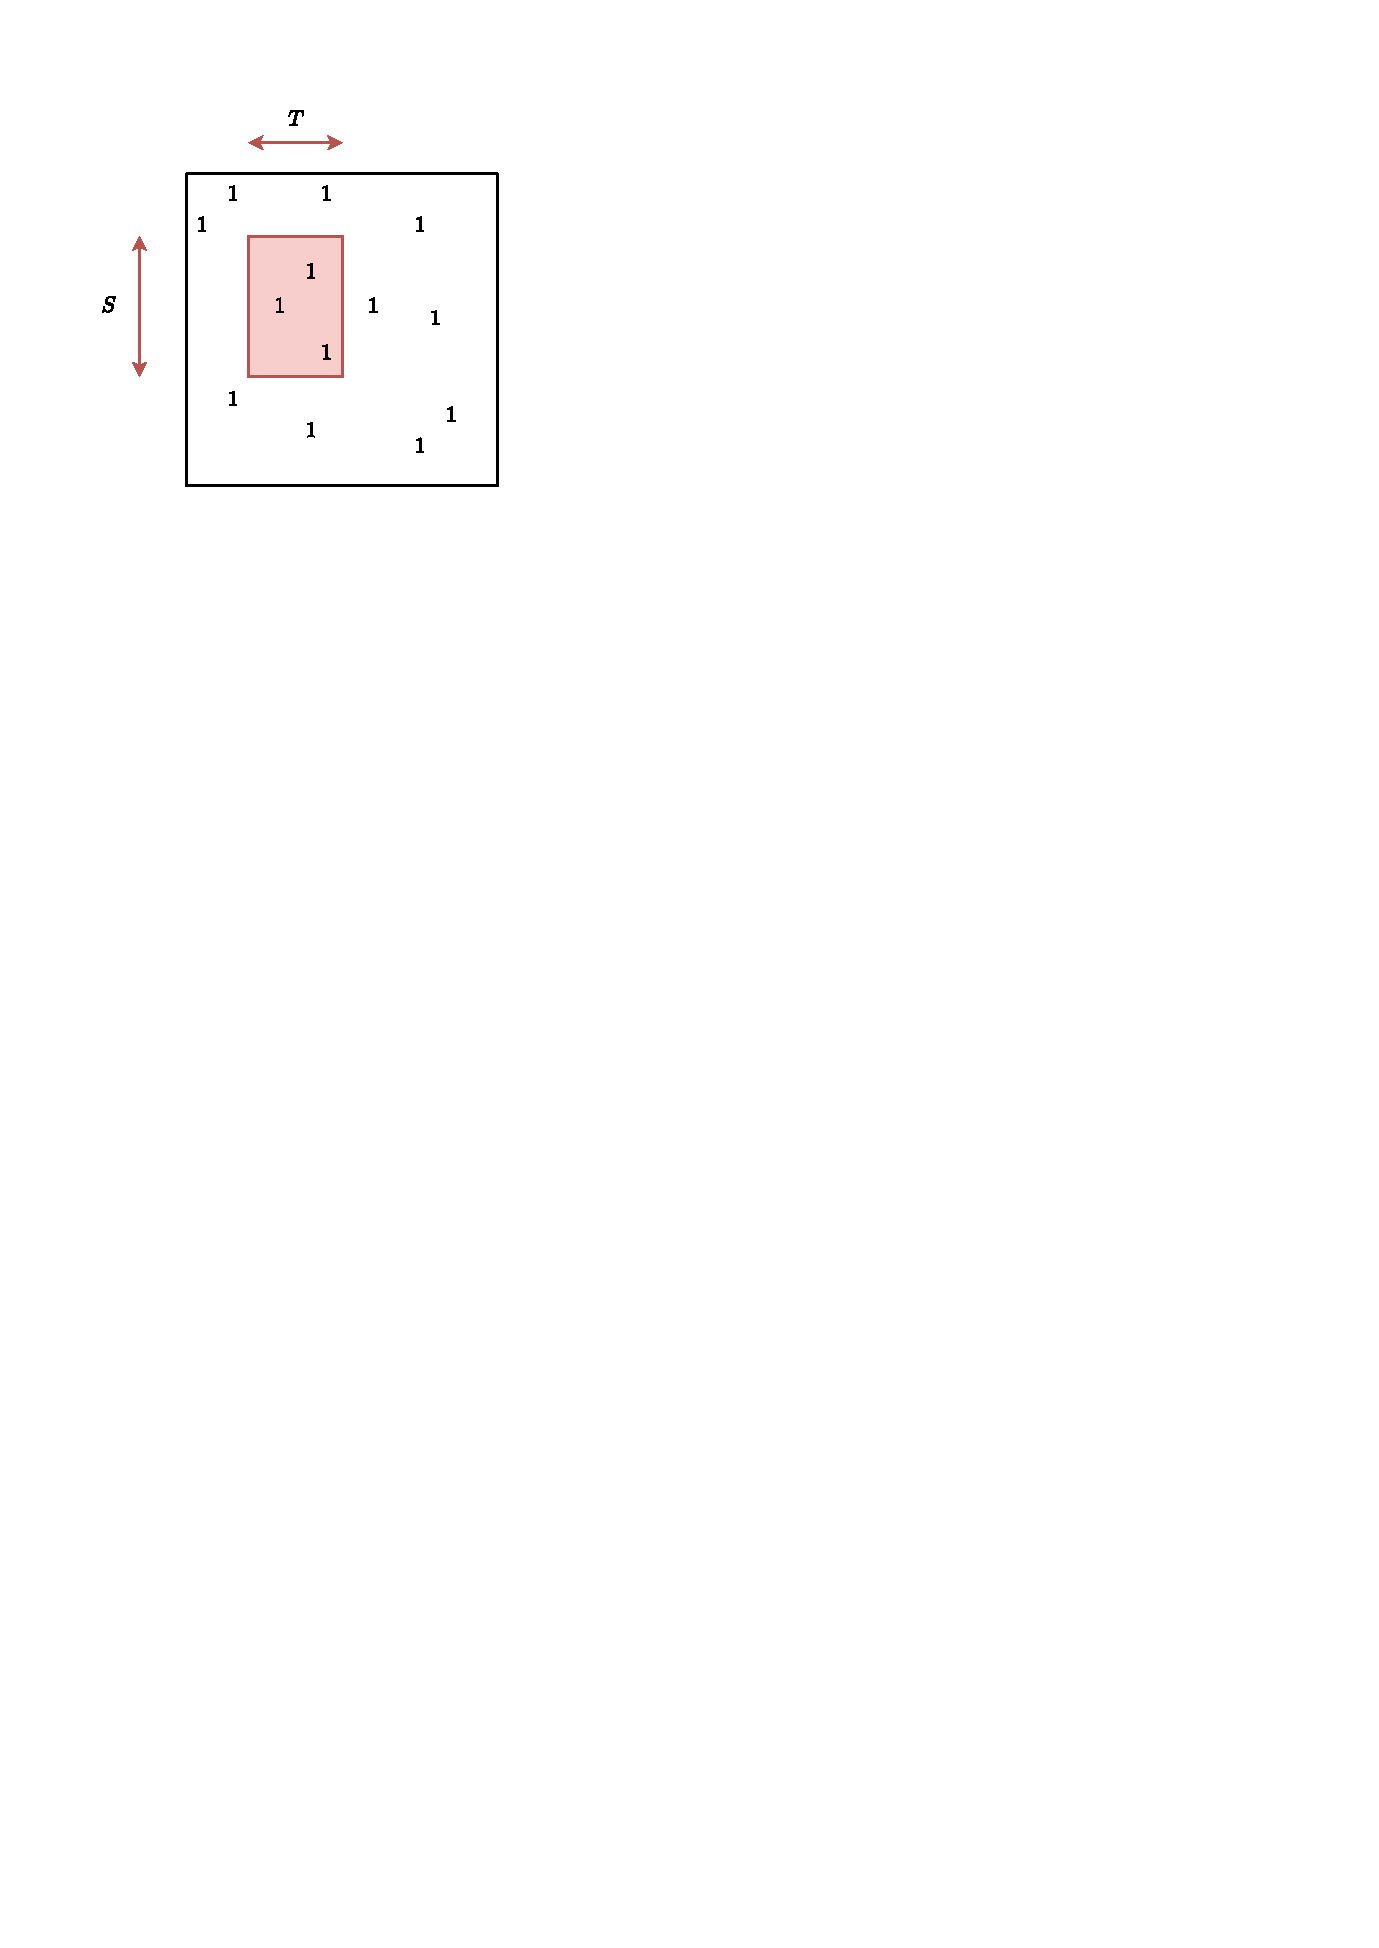
\includegraphics[width=6cm]{images/EML.pdf}
    \caption{正則グラフの隣接行列$A$を考える. このグラフがエクスパンダーならば, 頂点部分集合$S,T\subseteq V$で指定される長方形内に含まれる$1$の密度は行列全体の$1$の密度に近い値をとる. \label{fig:EML}}
    \end{center}
\end{figure}
%
\begin{proof}[\cref{lem:expander mixing lemma}の証明.]
    グラフ$G$上の単純ランダムウォーク$P$を考える.
    部分集合$S,T\subseteq V$に対し
    関数$f=\delta_S,g=\delta_T$として
    \cref{cor:general expander mixing lemma}を適用すると
    \begin{align*}
        &\piprod{f,Pg} = \frac{e(S,T)}{nd}, \\
        &\Epi f = \frac{|S|}{n},\\
        &\Epi [Pg] = \Epi g = \frac{|T|}{n},\\
        &\Varpi f = \frac{|S|}{n}\rbra*{1-\frac{|S|}{n}}, \\
        &\Varpi g = \frac{|T|}{n}\rbra*{1-\frac{|T|}{n}}
    \end{align*}
    より整理すると主張を得る.
\end{proof}

\begin{exercise}{}{check}
    \cref{lem:expander mixing lemma}の証明で表した五つの等式を実際に確認せよ.
\end{exercise}


\section{エクスパンダーグラフの応用} \label{sec:expander graph application}
グラフのエクスパンダー性は組合せ論的な興味だけでなく,
理論計算機科学において多くの定理の証明の道具として非常に重要な役割を果たしている.
ここではその一端を軽く紹介する.
より詳細の議論は\cite{HLW06}を参照されたい.
%
\subsection{脱乱択化}
Albert Einsteinは「量子は確率的に振る舞う」とする量子力学の枠組みに対して懐疑的であり,
1926年にMax Bornに宛てた手紙において
\begin{quotation}
    Der Alte würfelt nicht. (神はサイコロを振らない)
\end{quotation}
と述べている.
では, アルゴリズムの神はサイコロを振るだろうか?
より具体的には, 乱択は計算能力を真に向上させるだろうか?
この哲学的な問いは90年代から今もなお計算量理論において深く研究されており,
その中心的なリーダーの一人であるAvi Wigdersonは2021年にAbel賞, 2023年にTuring賞を受賞している.

ここではエクスパンダーグラフを使って「少ないサイコロで多くのサイコロの出目をhitting性の意味で模倣できる」
という結果を紹介する.
要素数$n$の集合$V$を考え, 頂点部分集合$U\subseteq V$を考える.
この集合$U$は「あたり」の集合とする.

\begin{comment}
話の分かりやすさのために多変数多項式の合同性判定(polynomial identity testing)を例に説明する.
有限体$\Fq$上の$n$変数$d$次多項式$f\colon \Fq^n\to \Fq$が恒等的に$0$かどうか (すなわち, 任意の$x\in\Real^n$に対し$f(x)=0$か否か) を判定したい\footnote{多項式合同性判定は二つの多項式$f,g$が恒等的に同じかどうかを判定する問題だが, $f-g$を考えればこの問題に帰着できる.}.
ただし有限体$\Fq$のサイズ$q$は十分大きく, 特に$\Fq>2d$を仮定する.
また, ここでは多項式$f$の次数をいわゆる全次数(total degree)で定義する.
すなわち$f(x_1,\dots,x_n)$に対しその次数$\deg f$を一変数多項式$x \mapsto f(x,\dots,x)$の最大次数として定義する.
関数$f$は\emph{オラクル}として与えられると仮定する.
すなわち, 「$x\in\Fq^n$に対して$f(x)$は何ですか?」と質問し, その答えを得ることができる.
できるだけ少ない回数の質問で$f$と$g$が恒等的に同じかどうかを判定するにはどうすればよいか?

この問題はランダムネスを許せば効率的に解ける.
次の補題を証明する.
\begin{lemma}{Schwartz--Zippelの補題}{Schwartz--Zippel}
    有限体$\Fq$上の$n$変数$d$次多項式$f \colon \Fq^n \to \Fq$が非ゼロ (ある$x\in\Fq^n$が存在して$f(x)\neq 0$) ならば,
    \[ \Pr_{x \sim \Fq^n} \sbra*{ f(x) = 0} \le \frac{d}{q}. \]
\end{lemma}
従って, 例えば$q \ge 2d$ならば, 一様ランダムな$x\sim\Fq^n$に対して$f(x)$が非ゼロかどうかを確認すれば確率$1/2$で正しくこの問題を解ける.

この乱択アルゴリズムは$x\sim\Fq^n$を乱択しているため, $n\log_q 2$ビットのランダムネスを用いている.
実は, エクスパンダーグラフを用いることでこのランダムビットの長さを減らすことができる.

\end{comment}

\subsection{誤り訂正符号}

\subsection{PCP定理}

\subsection{Goldreichの擬似乱数生成器}

\subsection{エクスパンダーハッシュ}

\section{Bibliographic Note}
